\chapter{Case-studie: Avstandsoppfølging i Trondheim kommune}
\label{ch:case}

\section{Innsamling av data}
Materialet i dette kapittelet er hovedsaklig basert på et gruppeintervju gjort med Renate Enger og Ingar Børre Sandvik med besøk
av en fastlege. Dette intervjuet ble gjennomført 24. mars 2017 fra kl. 09.00 til kl. 10.50 i lokalene til Trygghetspatruljen i
Trondheim kommune i Klæbuveien. Den formelle henvendelsen til velferdsteknologiprogrammet i Trondheim kommune er vedlagt i
tilegg \ref{appendix:formell}, og intervjuhendelsen er vedlagt i tillegg \ref{appendix:invitasjon_evaluering}. Temaene og
de forhåndsskrevne spørsmålene til intervjuet ligger i vedlegg \ref{appendix:forberedelse}.
Noe materiale fra evalueringsintervjuene gjort med SINTEF og Trondheim kommune i mai er
også med. Hvordan disse intervjuene ble gjennomført er nøyere beskrevet i kapittel \ref{ch:evaluation1}.

Trondheim kommune ga forskningsprosjektet en bruker til testmiljøet til løsningen de kjører. De viste også fram
nettbrettet som brukerne får utdelt. Dette, og informasjonen som allerede ligger tilgjengelig på nettet er en del
av dokumentdelen som analyseres.
%Koding: kategorier/temaer

\section{Bakgrunn og tjenesteforløp}
I følge I. B. Sandvik (personlig kommunikasjon, 24. mars, 2017), ble Trondheim kommune valgt ut til å delta i avstandsoppfølgingsprosjektet hovedsaklig fordi de hadde et
prosjekt tidligere som het \textit{HelsaMi} der ti KOLS-pasienter ble fulgt opp hjemme. I dette prosjektet var det ikke noen sensorer involvert,
kun mulighet til å rapportere dagsform med et nettbrett. Nåværende avstandsoppfølgingprosjekt er en fortsettelse av det arbeidet
og kalles for \textit{HelsaMi+}.

Kriteriene for å få tilbud om uttestingen er å ha KOLS eller hjertesvikt, være bosatt i en av kommunene som har tilbudet og ikke være så kognitivt
svekket at man ikke har nytte av teknologien. Det starter som oftest med en henvendelse til Helse- og velferdskontoret i kommunen som deretter
henviser videre til HelsaMi+. Noen henvisninger kommer også direkte til HelsaMi+, eller fra samarbeidskommuner. HelsaMi+ vurderer om det er en aktuell
bruker og tar en telefonsamtale til brukeren. Om de fortsatt er interesserte, avtaler HelsaMi+ et møte hos fastlegen der det blir utarbeidet en
egenbehandlingsplan i samråd med bruker, en representant fra HelsaMi+ og fastlegen. I etterkant av møtet avtales det et nytt tidspunkt for
hjemmebesøk der man får utstyr og opplæring i bruk av utstyret (R. Enger, 24. mars, personlig kommunikasjon).

Et moment er det målbare med tjenesten, nemlig i hvor stor grad man kan foregripe og redusere innleggelser på sykehus. Et annet moment er om man kan
øke trygghet- og mestringsfølelsen til brukerne. R. Enger sier at de ønsker at HelsaMi+ skal være et lavthengende kontaktpunkt. Mange tar kontakt
med legen altfor sent og det fører ofte til en innleggelse. Erfaringene viser at brukerne ikke forbinder et nettbrett med en
helsetjeneste: \textquote{De føler at kommunen er i kulissen, men det er lite inngripende i hverdagen}{.} Det kan gjøre at de mestrer
hverdagen bedre gjennom den følte tryggheten. Om fastlegene sier R. Enger dette: \blockquote{Fastlegen sier litt forskjellig om hva de tenker og mener
om det her. Men de aller fleste sier at de ser de kroniske syke for sjeldent. De er ikke flinke nok til å bestille time -- det
er en ting som er spilt inn veldig. vi driver og skal videreutvikle den
egenbehandlingsplanen nå. Og et av innspillene der er at legene ønsker å ha inn 'husk å ta de årlige vaksinene og bestill time til det'.}

Per 24. mars er det 65 brukere i løsningen og seks av disse har utplassert sensorer. Trondheim kommune har fått et ønsket måltall fra
ehelse-direktoratet på 150 til 200 brukere i løpet av året. Prisen på nettbrettet brukerne får utlevert er rundt 3000 kr. Videre koster
pulsoksimeter rundt 2000 kr, mens vekt og blodtrykksapparat koster rundt 1000 kr hver. Det gir i utgangspunktet en total sum på ca. 7000 kr
for et nettbrett med tre sensorer. Kommunen eier SIM-kortet som står i nettbrettet og betaler for all datatrafikken. I. B Sandvik sa at
det for kommunen er en ganske stor administrativ byrde å eie masse SIM-kort, og at det er et moment som må være med i kostnadsvurderingen
av denne type tjenester. Det er Direktoratet for eHelse for som anbefaler at kommunen bør eie hele verdikjeden, i dette tilfellet nettbrett
og SIM-kort.

Trondheim kommune drifter de fleste tjenestene som for eksempel hjemmebesøk, helsevakta, avstandsoppfølging og responssenter med egne ressurser:
\textquote[I. B Sandvik, 24. mars, personlig kommunikasjon]{Trondheim kommune har jo en veldig tydelig politisk ledelse og forankring på å ha mesteparten av
    ansvaret for sin egne tjenester selv, altså inhouse}{.}
Dette skiller seg fra Oslo og Sarpsborg som har større grad av outsourcing av tjenestene. Han påpeker også at Trondheim kommune til dels skiller
seg fra andre kommuner ved å tenke på robuste tjenester på en helhetlig måte, og ikke bare på teknologien:
\blockquote[I. B Sandvik, 24. mars, personlig kommunikasjon]{For det som Trondheim kommune er
    veldig tydelige på, og kanskje til dels skiller oss fra andre kommuner når det gjelder velferdsteknologi -- det er at det er ikke teknikken og dingsene som på en måte skal
    løse alt. Det er tjenesten vi skal bygge som understøttes av teknologien.
    Vi ser jo det at det å kunne pilotere i småskala, med ny teknologi, det greier de fleste. Men det å bygge en robust tjeneste som skal implementeres i en stor kommune
-- det er noe helt annet. Og som skal da kunne rulles ut i storskala med mange hundre brukere av ulike tjenester.}


\section{HelsaMi+}
Brukeren har et nettbrett som kjører en androidapplikasjon. Denne applikasjonen pakker inn
et webgrensesnitt. I tillegg til hovedapplikasjonen er det en sensorhub-applikasjon som kjører i bakgrunnen
og har ansvaret for tilkoblingen til alle sensorene. Alle skjermbildene i dette delkapittelet er tatt i testmiljøet
til Trondheim kommune i en nettleser.

Beskrivelsen av løsningen og skjermbildene tar utgangspunkt i to scenarioer for sluttbrukere
og ett scenario for helsepersonell: for brukere er det å rapportere dagsform og utføre en måling med pulsoksimeter,
og for helsepersonell er det å gå inn for å se på hvilken data som er kommet inn.

Det første som møter brukeren er hovedskjermen i figur \ref{fig:helsami_hovedskjerm}. I testmodus er alle de ulike
alternativene vist.
Herfra kan brukeren trykke seg inn for å rapportere dagsform for \textit{KOLS} og \textit{HJERTESVIKT}, eller utføre en sensormåling med
enten vekt, blodtrykk eller pulsoksimeter. Det er også mulig å gå på \textit{Brukerveiledninger} for å få instruksjoner og hjelp.
For en bruker som har KOLS og en sensor utplassert hjemme, vil skjermen for eksempel vise KOLS og SpO2.

\begin{figure}
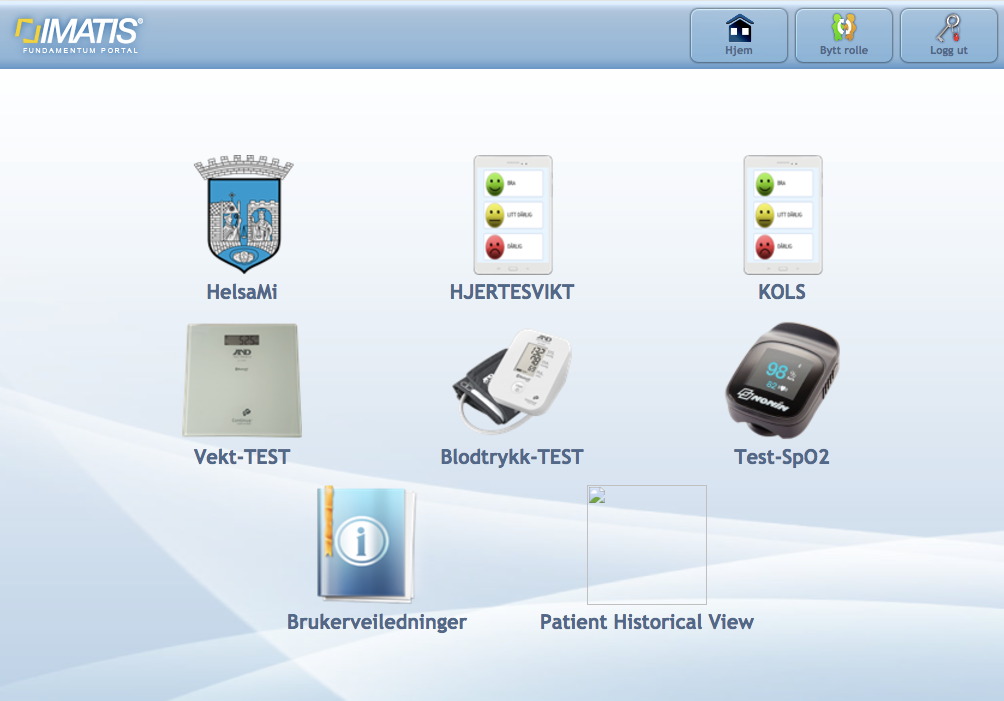
\includegraphics[width=1.0\textwidth,center]{fig/helsami/hovedskjerm}
\caption{HelsaMi+: Hovedskjerm}
\label{fig:helsami_hovedskjerm}
\end{figure}

\subsection{Rapportere dagsform}
Scenariet er at en bruker med KOLS skal rapportere dagsform. Brukeren trykker på KOLS på hovedskjermen,
og kommer til figur \ref{fig:helsami_kols_start}. Et klikk på \textit{Start} tar brukeren til \ref{fig:helsami_kols_sp1}.
Det er fire spørsmål brukeren svarer på. Alle svaralternativer som er subjektive spør brukeren om å sammenligne med
hvordan det er til vanlig.

\begin{itemize}
  \tightlist
  \item Hvordan er pusten din?
  \item Hvordan er hosten?
  \item Hvordan er fargen på oppspyttet ditt?
  \item Hvordan føler du deg til sinns?
\end{itemize}

Etter spørsmålene får brukeren mulighet til å legge inn en skriftlig kommentar og se over at det er greit
før alt sendes inn (figur \ref{fig:helsami_kols_sammendrag}). Brukeren får beskjed om at tilbakemeldingen er sendt,
og må selv aktivt klikke seg tilbake til menyen etterpå.

\begin{figure}
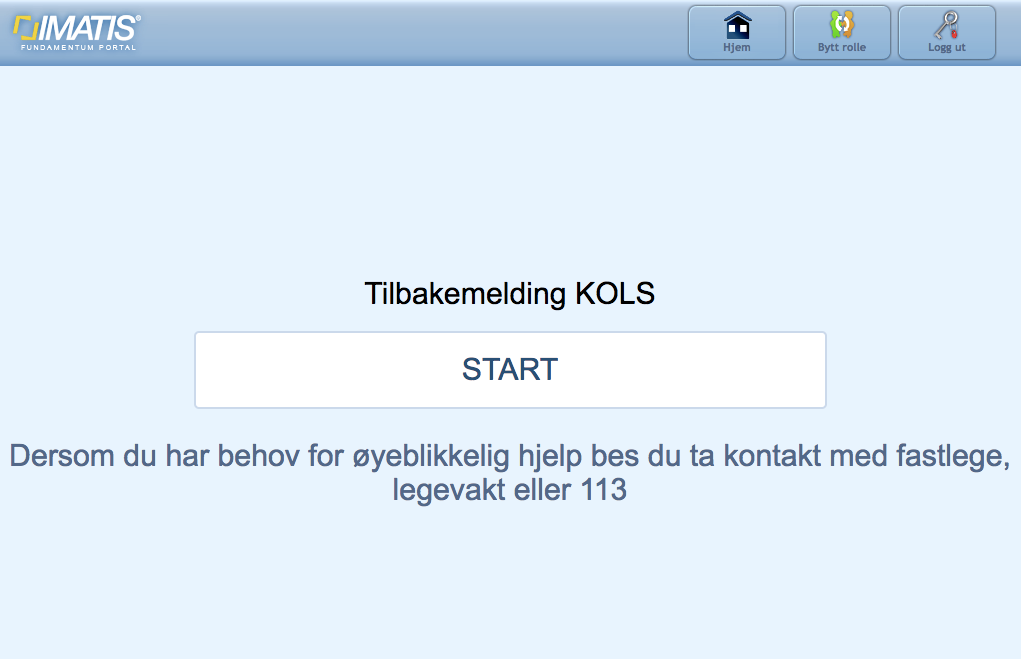
\includegraphics[width=1.0\textwidth,center]{fig/helsami/kols_start}
\caption{HelsaMi+: Tilbakemelding KOLS}
\label{fig:helsami_kols_start}
\end{figure}

\begin{figure}
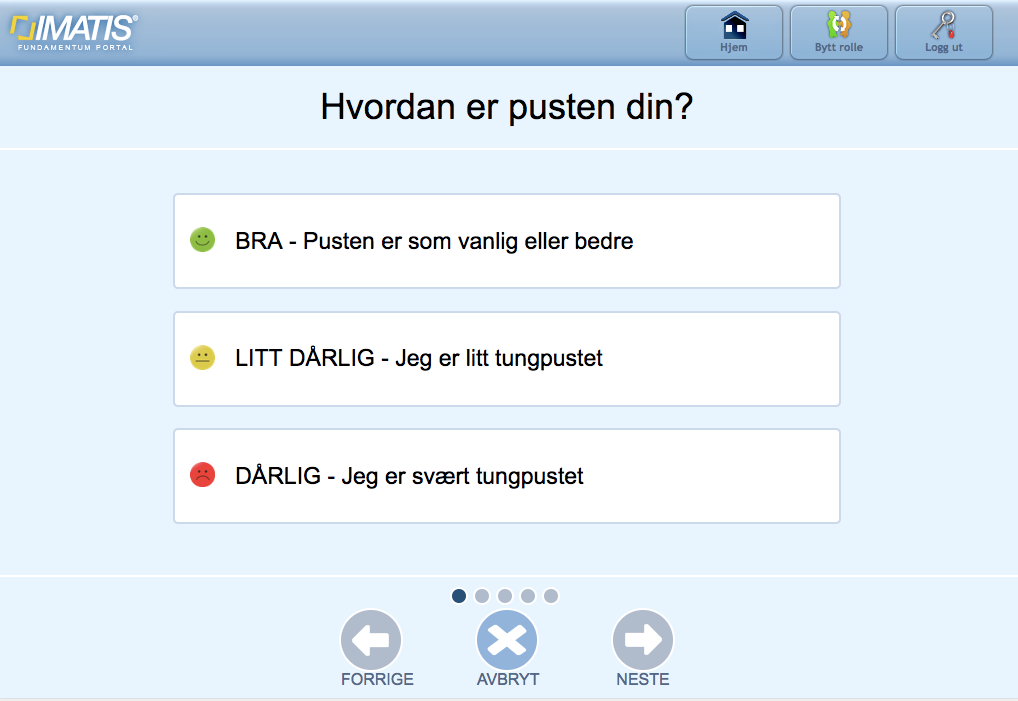
\includegraphics[width=1.0\textwidth,center]{fig/helsami/kols_sp1}
\caption{HelsaMi+: Spørsmål 1}
\label{fig:helsami_kols_sp1}
\end{figure}

\begin{figure}
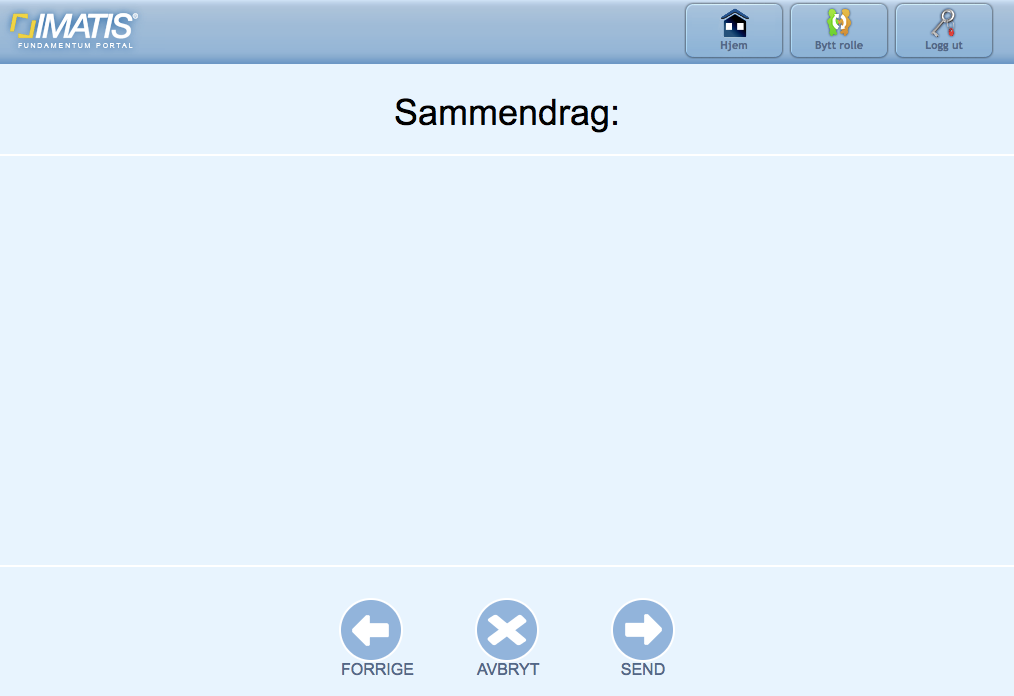
\includegraphics[width=1.0\textwidth,center]{fig/helsami/kols_sammendrag}
\caption{HelsaMi+: Sammendrag}
\label{fig:helsami_kols_sammendrag}
\end{figure}

\subsection{Utføre en måling med pulsoksimeter}
Et klikk på \textit{Test-SpO2} tar brukeren til en mellomskjerm med informasjon om at
brukeren ikke har utført en måling ennå med et bilde av sensoren. Brukeren klikker seg videre
til en skjerm med to valg, enten \textit{Trykk her for å måle oksygenmetning og puls} eller \textit{Trykk her for brukerveiledning}
(figur \ref{fig:helsami_pulsoksimeter_oversikt}). Det første valget tar brukeren til figur \ref{fig:helsami_pulsoksimeter_maaling}
der brukeren klikke på en knapp og setter måleren på fingeren. Brukeren må ha en gyldig sensorhub installert for
å få lov til å gjennomføre en måling.

\begin{figure}
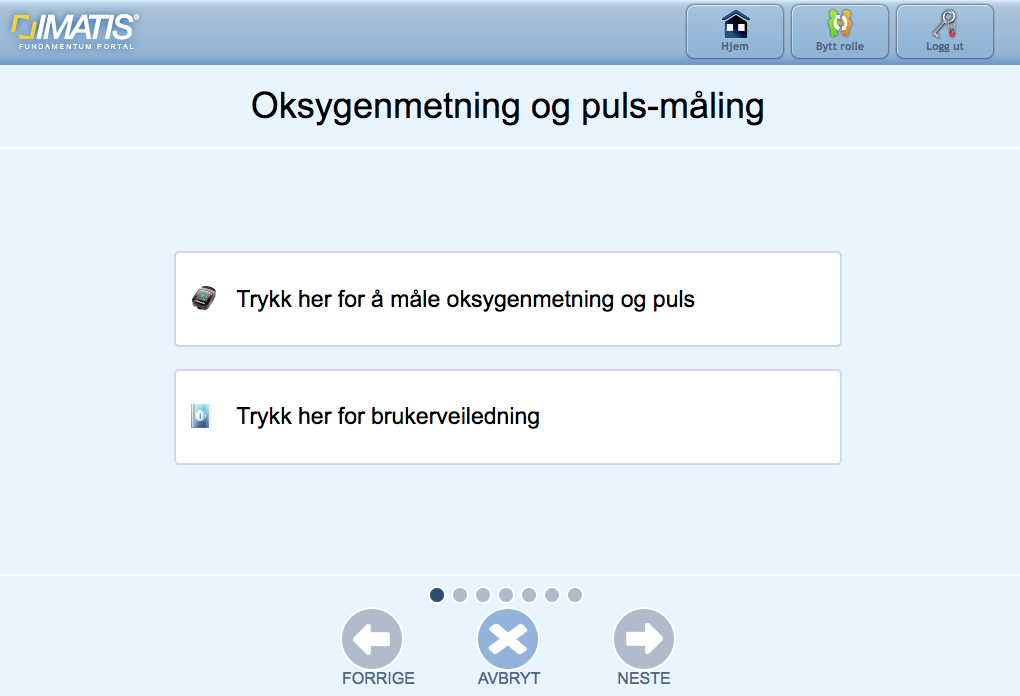
\includegraphics[width=1.0\textwidth,center]{fig/helsami/pulsoksimeter_oversikt}
\caption{HelsaMi+: Pulsoksimeter-oversikt}
\label{fig:helsami_pulsoksimeter_oversikt}
\end{figure}

\begin{figure}
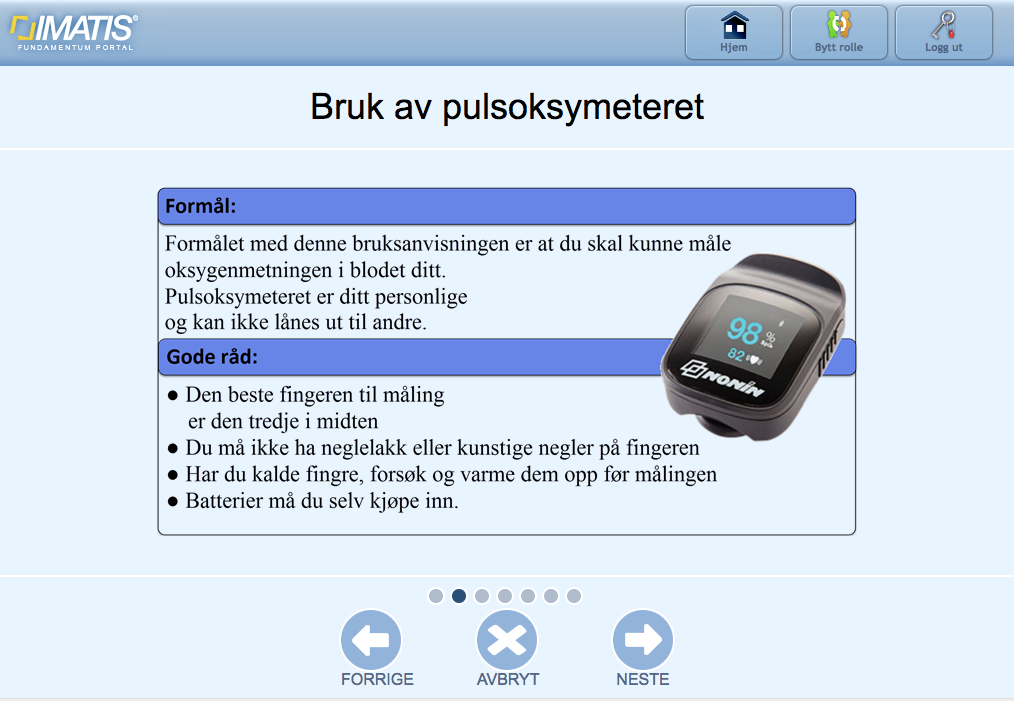
\includegraphics[width=1.0\textwidth,center]{fig/helsami/pulsoksimeter_veiledning}
\caption{Pulsoksimeter-veiledning}
\label{fig:helsami_pulsoksimeter_veiledning}
\end{figure}

\begin{figure}
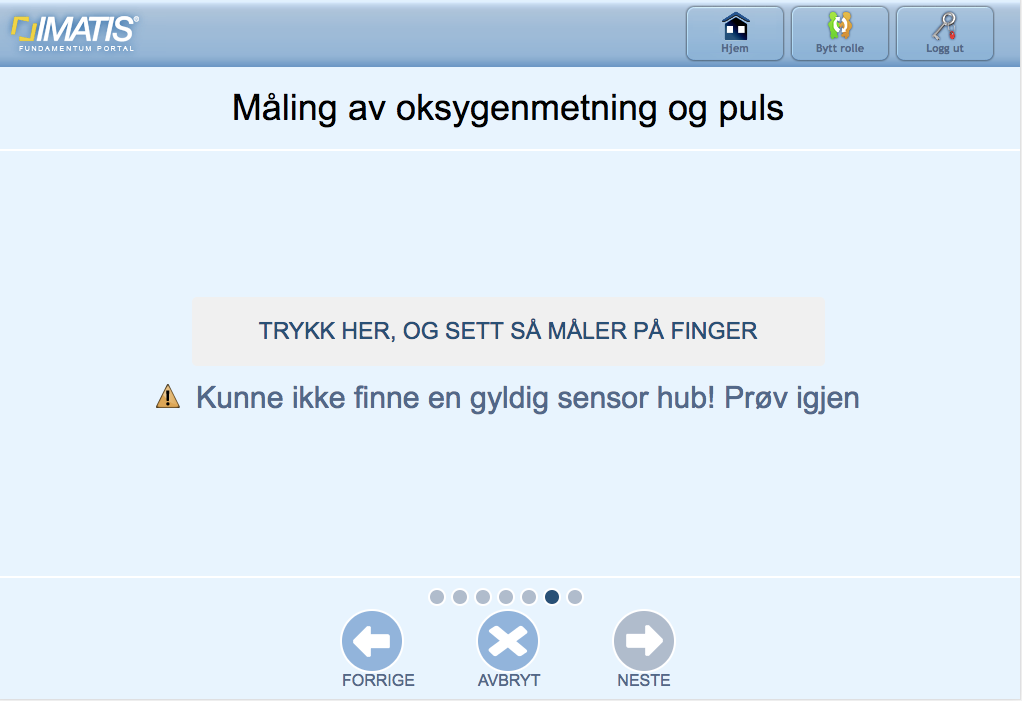
\includegraphics[width=1.0\textwidth,center]{fig/helsami/pulsoksimeter_maaling}
\caption{HelsaMi+: Pulsoksimeter-måleskjerm}
\label{fig:helsami_pulsoksimeter_maaling}
\end{figure}

\subsection{Se på innrapport data}
Trykk på \textit{HelsaMi}. Figur \ref{fig:helsami_admin1} viser hvordan oversikten over innrapportert data ser ut.

\begin{figure}
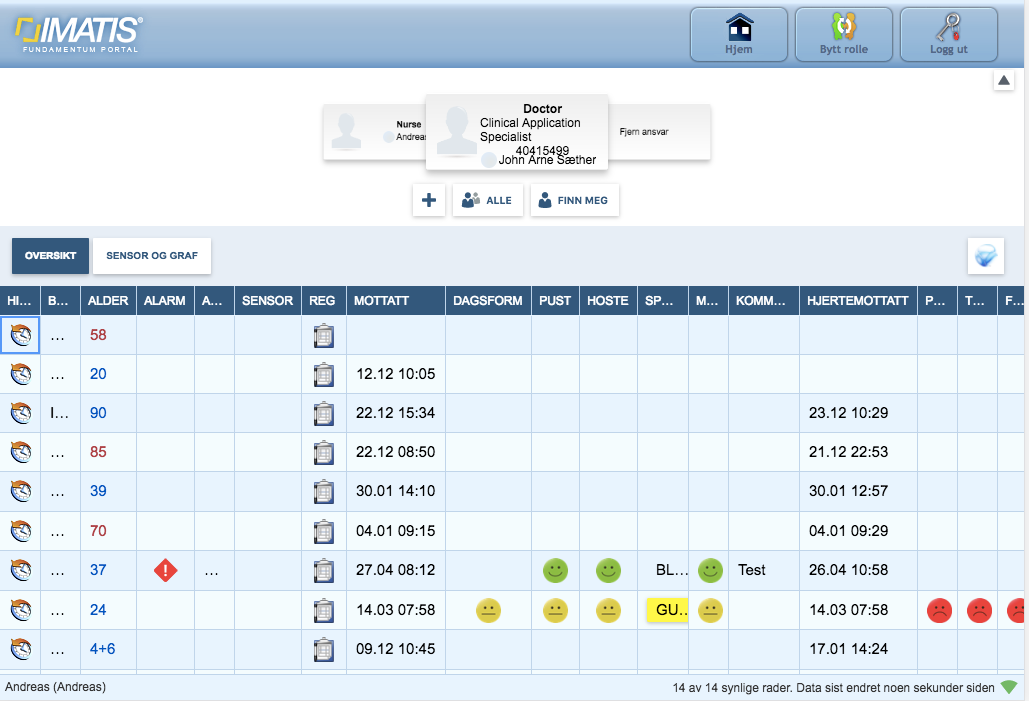
\includegraphics[width=1.0\textwidth,center]{fig/helsami/admin_oversikt}
\caption{HelsaMi+: Oversikt for administrator 1/2}
\label{fig:helsami_admin1}
\end{figure}

\section{Utfordringer og refleksjoner}
I. B Sandvik (personlig kommunikasjon, 23. mars, 2017) påpekte at den største utfordringen med prosjektet ikke er teknologien, men samhandlingen mellom de ulike
helseinstansene:

\blockquote{Det som er interessant med denne uttestingen av tjenesten er jo å se hvilke gevinster, for det er jo gevinster man ønsker å kartlegge, hvilke gevinster man tror
    man kan få med å drive med den type ny helsetjeneste med oppfølging av brukere mens de bor hjemme. og det som gjør prosjektet her så relativt komplekts -- en ting
    er jo den teknologiske delen -- det er jo stort sett håndterbart. Dette er jo et prosjekt som går på tvers av kommune, fastlege og spesialisthelsetjeneste. Det vil
si midt inne i samhandlingsreformdomenet.}

De ulike helseinstansene har forskjellige former for måloppnåelse og egne budsjetter. De statlige helseforetakene har ansvaret for sykehusene,
ikke kommunen. I. B Sandvik forklarer hvorfor dette kan være en utfordring:

\blockquote{Det er jo en utfordring av mange grunner. Både på grunn av kultur, fokus. Spesialister er jo diagnoserettet, kommunen har jo det hele mennesket som fokus. Og
    fastlegen sitter jo der i mellom og skal egentlig ha ansvaret og kontroll over alt som foregår over sine pasienter mens de er utenfor sykehuset sitt domene. Så det er
    mange interessante problemstillinger som har blitt avdekket. Blant annet det vi kan nevne et par eksempler det med det juridiske: hvem skal ha ansvaret for hva,
    hvordan skal opplysninger deles mellom partene -- ikke rett frem. Det andre er dette med finaniseringsmodellene. Det er jo ikke noe tvil om at den største investeringen
    i denne type tjeneste gjøres av kommunen, når det gjelder å rigge tjeneste, oppfølging, utstyr, alt dette her. Mens gevinstene kanskje i større
grad tas ut på sykehuset, med færre innleggelser.}

I. B Sandvik reflekterte også rundt den juridiske problematikken med avstandsoppfølging relatert til personvernet:
\blockquote{(...) og en annen dimensjon også der som går på det juridiske for at -- et spørsmål rundt dette med egenmålinger og rapportering er
'hva trenger på en måte kommunen å vite'. I teorien så trenger vi egentlig bare å vite det som gir et grunnlag til en vurdering og tiltak.
Og der er jo den juridiske vurderingen 'hvem skal eie og sitte på dataen' og per i dag så får vi jo alt innrapportert og har tilgang på
all informasjon i den her løsningen.}

Konklusjonen per i dag fra Trondheim kommune sin side er at så lenge fastlegen vurderer at dataen som kommer inn er relevant, så er det innenfor
regelverket. Utgangspunktet nå er at alle som får egenbehandlingsplan av fastlegen er vurdert som relevante for å sende inn måledata. I samtalen
med I. B Sandvik kom man inn på at det kun er målinger som blir identifisert som i faresonen (røde målinger) som skal føre til et tiltak fra
kommunen sin side, mens grønne målinger er greie. Skal man da lagre de grønne målingene?
Spørsmålet er om de grønne målingene kan være nyttige i en trendanalyse av dataene.
I dag blir alle målinger lagret av kommunen i løsningen.

I. B sa at det er teknologisk forbedringspotensiale på at brukeren skal finne
ut hvilken data som er samlet inn og styre sin egen data på en bedre måte. Dette er ikke implementert i løsningen til Trondheim kommune i dag,
men blir enda mer relevant med ny personvernslov.
